\documentclass[8 pt]{article}

\usepackage[utf8x]{inputenc}
\usepackage{dsfont}
\usepackage{amsthm}
\usepackage{amsfonts}
\usepackage{amssymb}
\usepackage{tensor}
\usepackage{mathtools}
\usepackage[T1]{fontenc}
%\usepackage[spanish]{babel}
\usepackage[cm]{fullpage}
\usepackage{graphicx}
%\usepackage{float}
\usepackage{bm}
\usepackage{setspace}
\usepackage{enumitem}
\usepackage{mdwlist}
\usepackage{parskip}
\usepackage{listings}
\usepackage{color}
%\usepackage{epstopdf}
\usepackage{tikz,datatool}
\usepackage{hyperref}
\usepackage{mathabx}
\usepackage{multicol}
\usepackage{eurosym}
\usepackage{caption}

\newcommand{\HRule}{\rule{\linewidth}{0.5mm}}

\AtBeginDocument{
  \let\myThePage\thepage
  \renewcommand{\thepage}{\oldstylenums{\myThePage}}
}

\newcommand{\gra}{$^\text{o}$}
\newcommand{\dif}{\text{d}}
\newcommand{\avg}[1]{\left\langle #1 \right\rangle}
\newcommand{\ket}[1]{\left| #1 \right\rangle}
\newcommand{\bra}[1]{\left\langle #1 \right|}
\newcommand{\bket}[2]{\left\langle #1 \middle| #2 \right\rangle}
\newcommand{\der}[2]{\frac{\text{d} #1}{\text{d} #2}}
\newcommand{\prt}[2]{\frac{\partial #1}{\partial #2}}
\newcommand{\dert}[3]{\frac{\text{d}^#3 #1}{\text{d} #2^#3}}
\newcommand{\prtt}[3]{\frac{\partial^#3 #1}{\partial #2^#3}}
\newcommand{\dl}{\mathcal{L}}
\newcommand{\dha}{\mathcal{H}}
\newcommand{\vol}{\text{vol}}
\renewcommand{\vec}[1]{\pmb{#1}}

\DeclarePairedDelimiter\ceil{\lceil}{\rceil}
\DeclarePairedDelimiter\floor{\lfloor}{\rfloor}

\newenvironment{Figure}
  {\par\medskip\noindent\minipage{\linewidth}}
  {\endminipage\par\medskip}

\begin{document}

\begin{minipage}{\textwidth}
    \centering
    \Large \textbf{\textsc{Homework 2: Sensitivity and Option Strategies}}
    \vspace{0.5cm}

    \small \textsc{Francisco García Flórez, Joris van Lammeren, Wouter Varenkamp}
    \vspace{0.5cm}

    \begin{minipage}{0.6\textwidth}
      \textbf{Abstract.} In this exercise we continue using the program written for the last homework, analyzing now the sensitivity of the option prices to changes in several parameters. In the second part, we analyze the stategy \emph{long call option} and compute the \emph{put-call parity}.
    \end{minipage}
\end{minipage}

\vspace{0.5cm}

\begin{multicols*}{2}
\section{Sensitivity of the option price}

Firstly we will show how the option price is affected by changes in several variables of the Weiner process. In the following plots we show the mean and standard deviation values for each one, the second one using error bars. Also, the option price for call options will be shown in red, while the one for put options will be shown in blue.

Some comparisons can be done against the Black-Scholes model, which solves analytically the stochastic differential equation of the Weiner process, giving the following solution \cite{Wilmott} for the probability density function of S:

\begin{equation} \label{eq:weinersol}
  \frac{1}{\sigma S \sqrt{2\pi t}} \exp\left[ -\frac{\left(\log\frac{S}{S_0} - (\mu - \frac{1}{2}\sigma^2)t\right)^2}{2\sigma^2 t}\right] ~~,
\end{equation}

also known as lognormal distribution.

Just by looking at this equation we can predict the behavior of the option price as parameters change --- $\sigma$ and $t$, which will clearly widen the distribution of points as they increase, and $\mu$ or $S_0$ which will shift the whole distribution changing the option price but without affecting the width.

\subsection{Initial stock price, $S_0$}

\begin{Figure}
  \begin{center}
    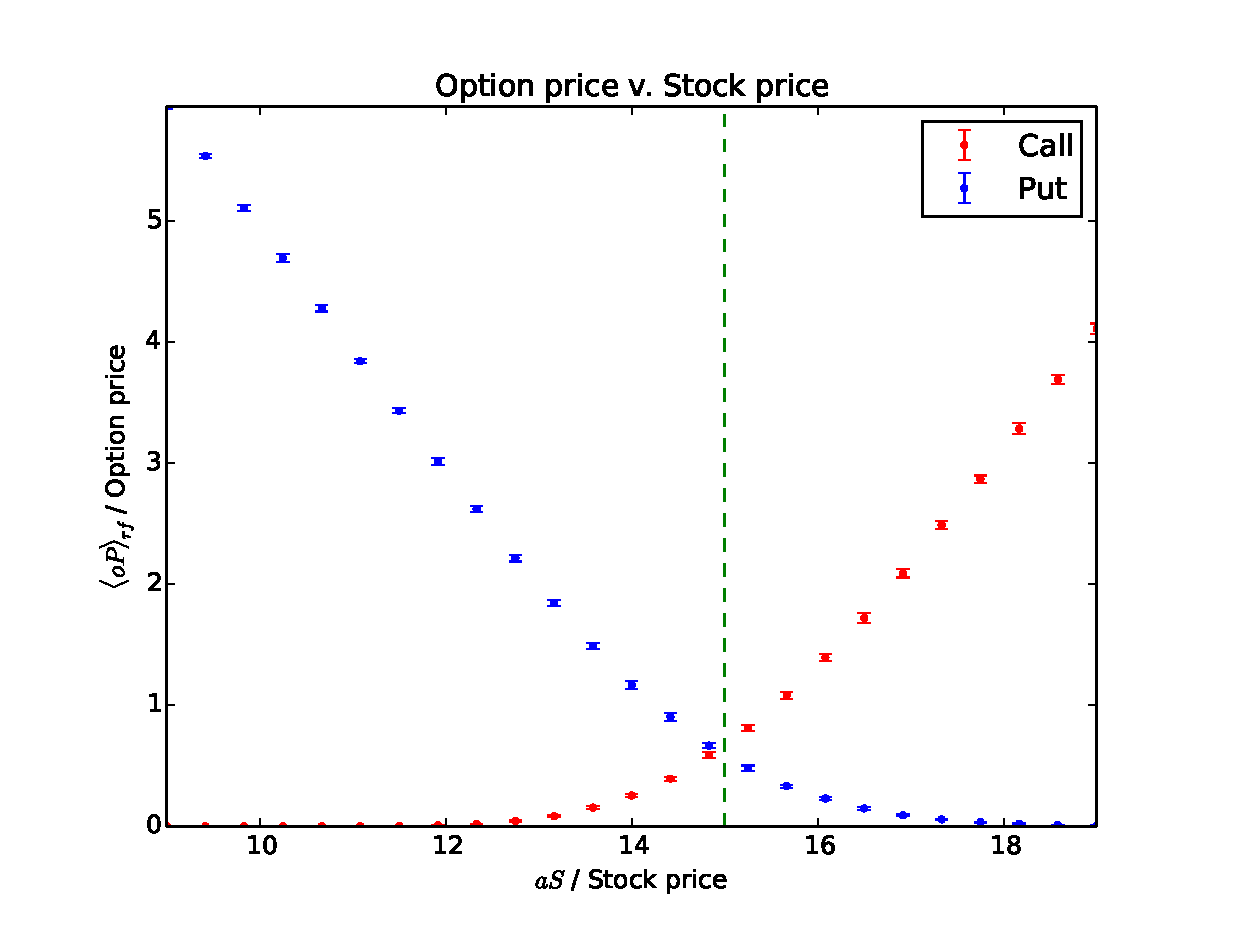
\includegraphics[width=0.8\textwidth]{graphs/oP_stock.eps}
    \captionof{figure}{Value and sensitivity of the option price for a range of initial stock prices. The green line represents the exercise price (15\euro).}
    \label{fig:stock_sens}
  \end{center}
\end{Figure}

As we can see in Figure \ref{fig:stock_sens}, changing the initial stock price doesn't affect the option price in an unexpected way, and the standard deviation of our results doesn't increase significantly either. This is expected, since what we are doing here is just moving the distribution of share value at exercise date to higher or lower values, so for lower (higher) values smaller (larger) the probability of making profit and therefore the option price will be lower (higher).

\subsection{Volatility, $\sigma$}

\begin{Figure}
  \begin{center}
    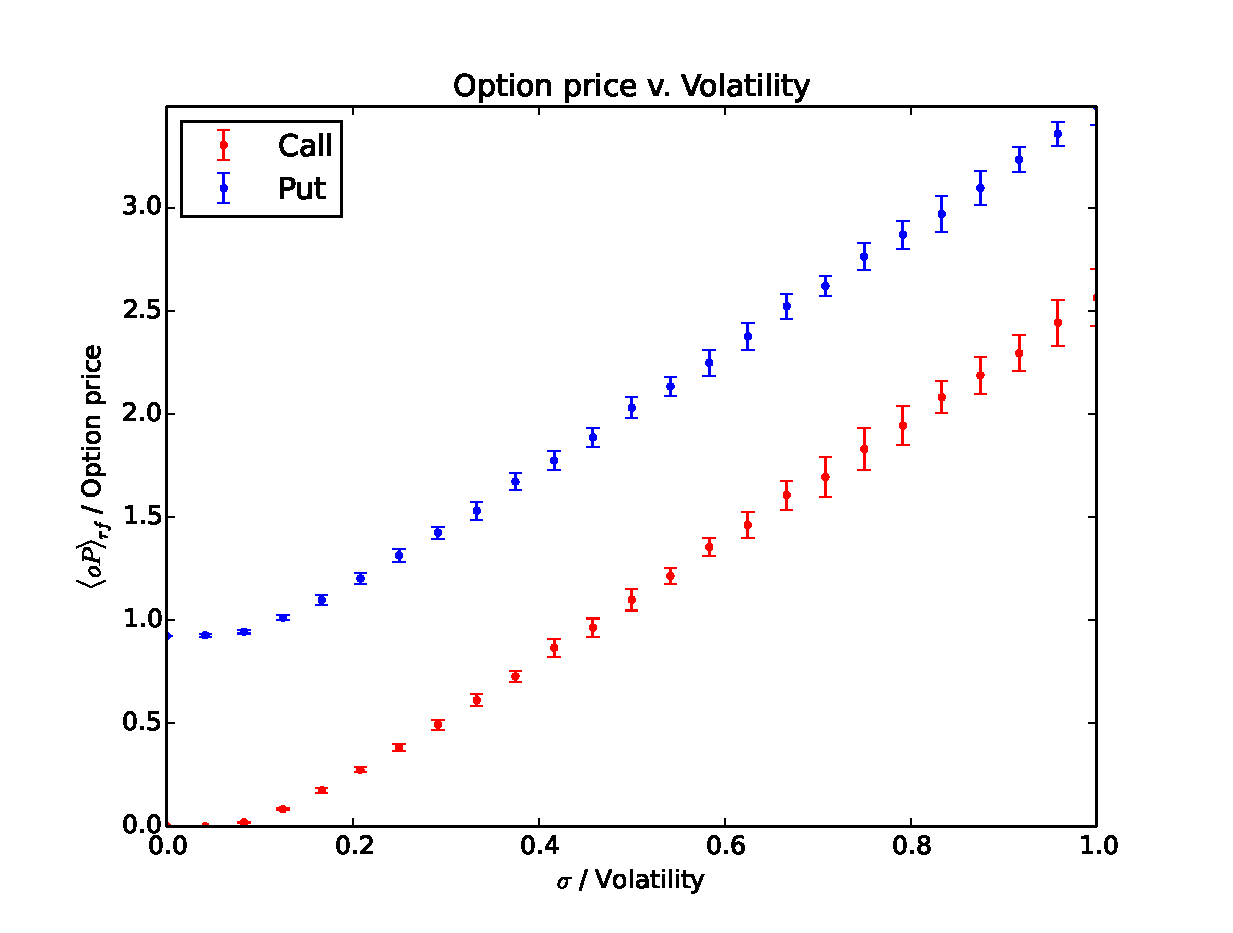
\includegraphics[width=0.8\textwidth]{graphs/oP_vol.eps}
    \captionof{figure}{Value and sensitivity of the option price for a range of volatilities.}
    \label{fig:vol_sens}
  \end{center}
\end{Figure}

In this case we are changing the volatility of the action, so its value at exercise date will have a wider range of values. In other words, we expect the standard deviation of our results to be larger as we can predict by looking at equation (\ref{eq:weinersol}). The denominator of the distribution is given by $2\sigma^2 t$, and it clearly explains this behavior. Also, for $\sigma\rightarrow0$ we find no width at all, since the values will only change due to the drift.

The option price is also increasing, since a higher volatility spreads the share value at expiration date, and since we compute the option price by removing values smaller than the exercise price, it increases the average.

\vfill

\subsection{Duration, $aT$}

\begin{Figure}
  \begin{center}
    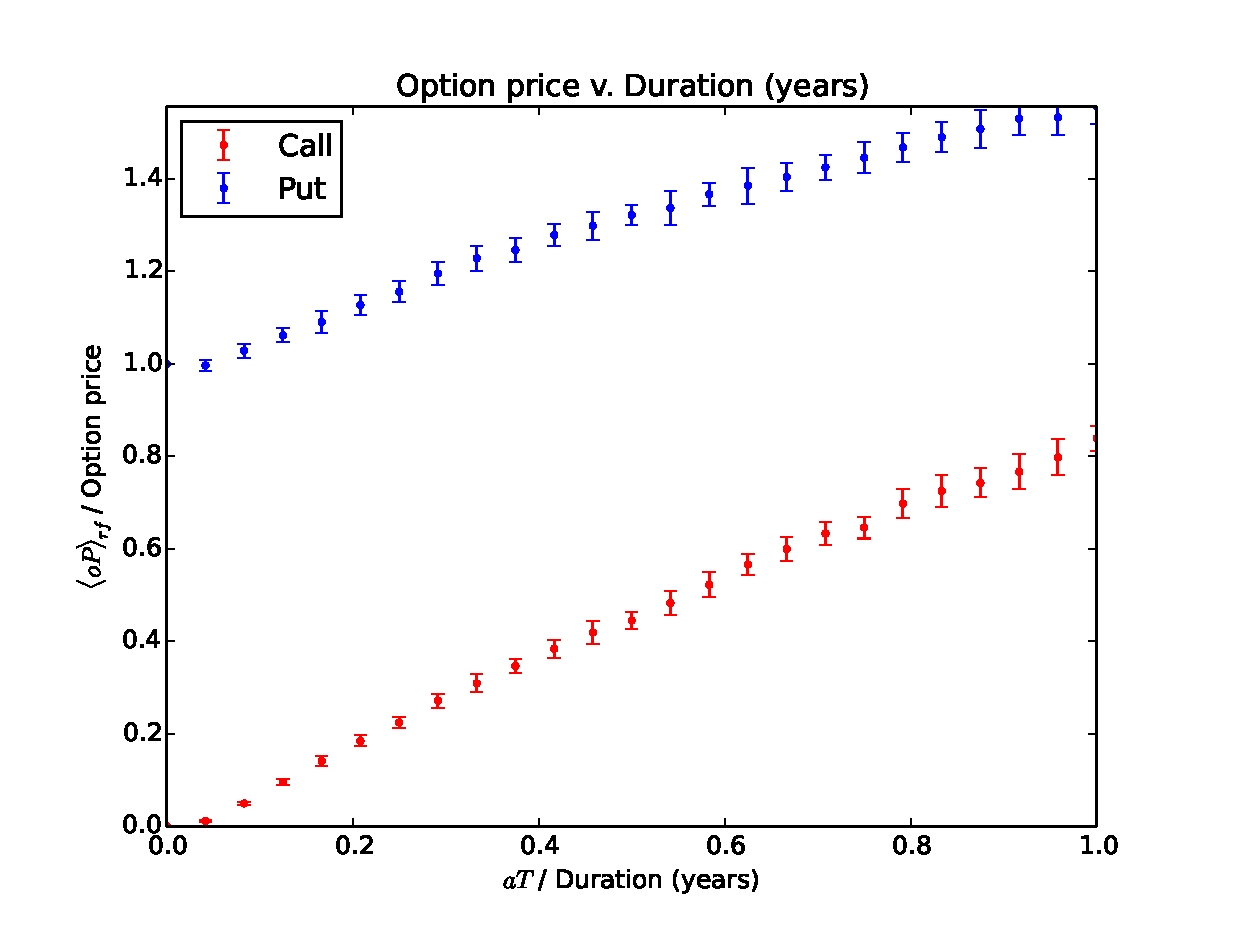
\includegraphics[width=0.8\textwidth]{graphs/oP_dur.eps}
    \captionof{figure}{Value and sensitivity of the option price for a range of durations.}
    \label{fig:dur_sens}
  \end{center}
\end{Figure}

Again, the error bars widen as $t$ increases, since the standard deviation depends on $\sqrt{t}$ as we can see from equation \ref{eq:weinersol}. Other than that, the option price increases, since the drift has more time to act and thus increase the value of the share. For large $t$ we should include a term of the form $e^{-rt}$, but we will just assume that $r$ is small enough not to make a significant difference in a year.

As we mentioned before, changing $aT$ is similar to a change in $\sigma$ in terms of widening of the distribution, and it shows clearly as Figures \ref{fig:vol_sens} and \ref{fig:dur_sens} both present a similar behavior, the former increasing $\avg{oP}_{rf}$ linearly and the latter as $\sqrt{t}$.

\subsection{Drift, $\mu$}

\begin{Figure}
  \begin{center}
    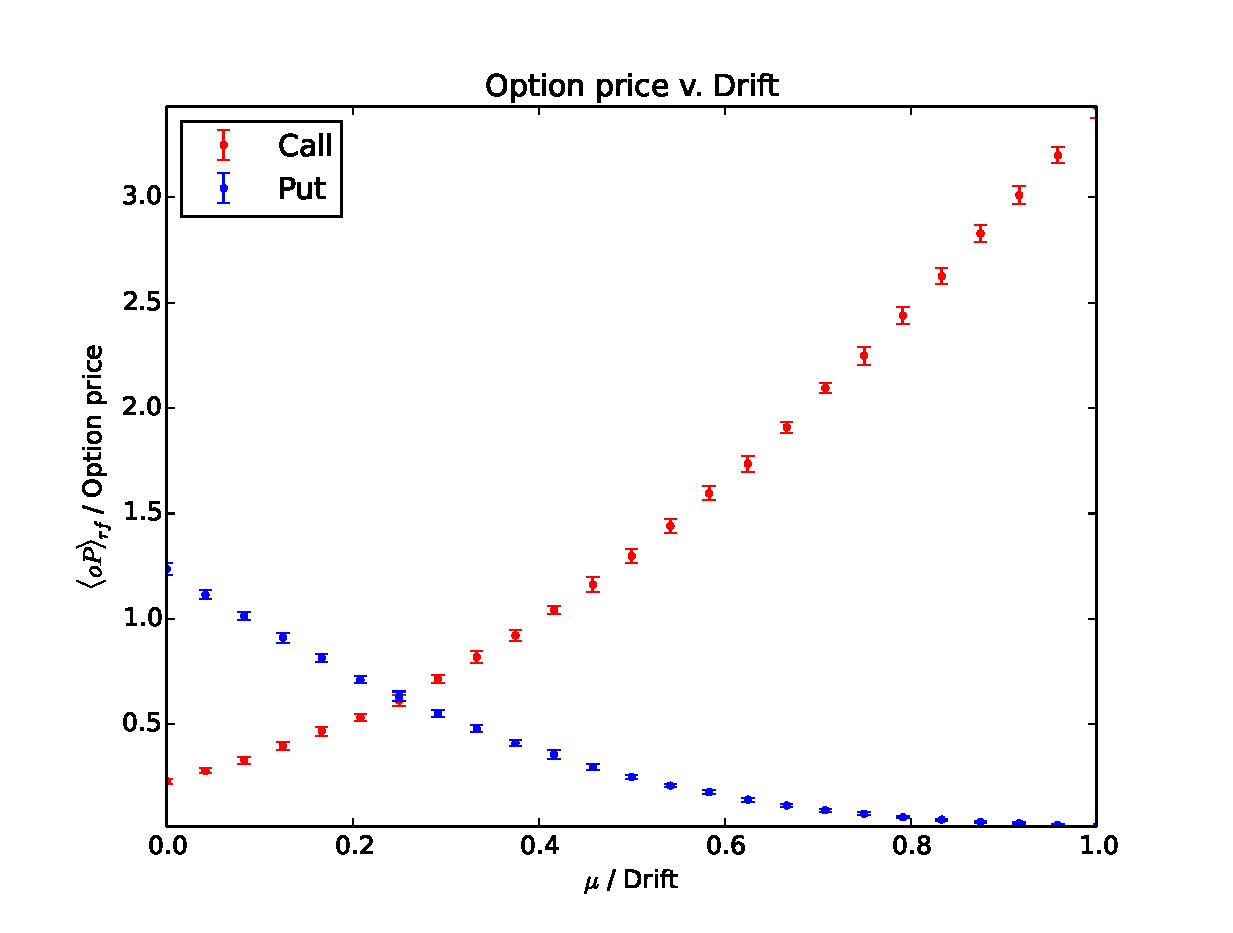
\includegraphics[width=0.8\textwidth]{graphs/oP_drift.eps}
    \captionof{figure}{Value and sensitivity of the option price for a range of drifts.}
    \label{fig:drift_sens}
  \end{center}
\end{Figure}

Finally, in Figure \ref{fig:drift_sens} we can see how changing the drift produces a very similar result as changing the initial stock price from Figure \ref{fig:stock_sens}, as we predicted by studying equation (\ref{eq:weinersol}). We could check that these two plots are equal when $\log S_0$ and $\mu t$ give the same contribution. Also as we predicted, the standard deviation doesn't significantly change with $\mu$, except for the inherent randomness of the algorithm.

\section{$A$/$B$ long call spread}

When using a long call spread you are buying a call option (going long) with a price $A$ and writing a call option (going short) with a price $B$. A is smaller than B and the stock price is usually in between but does not have to be. This limits the risk you are taking, but it also limits your profits to a maximum value.

\begin{Figure}
  \begin{center}
    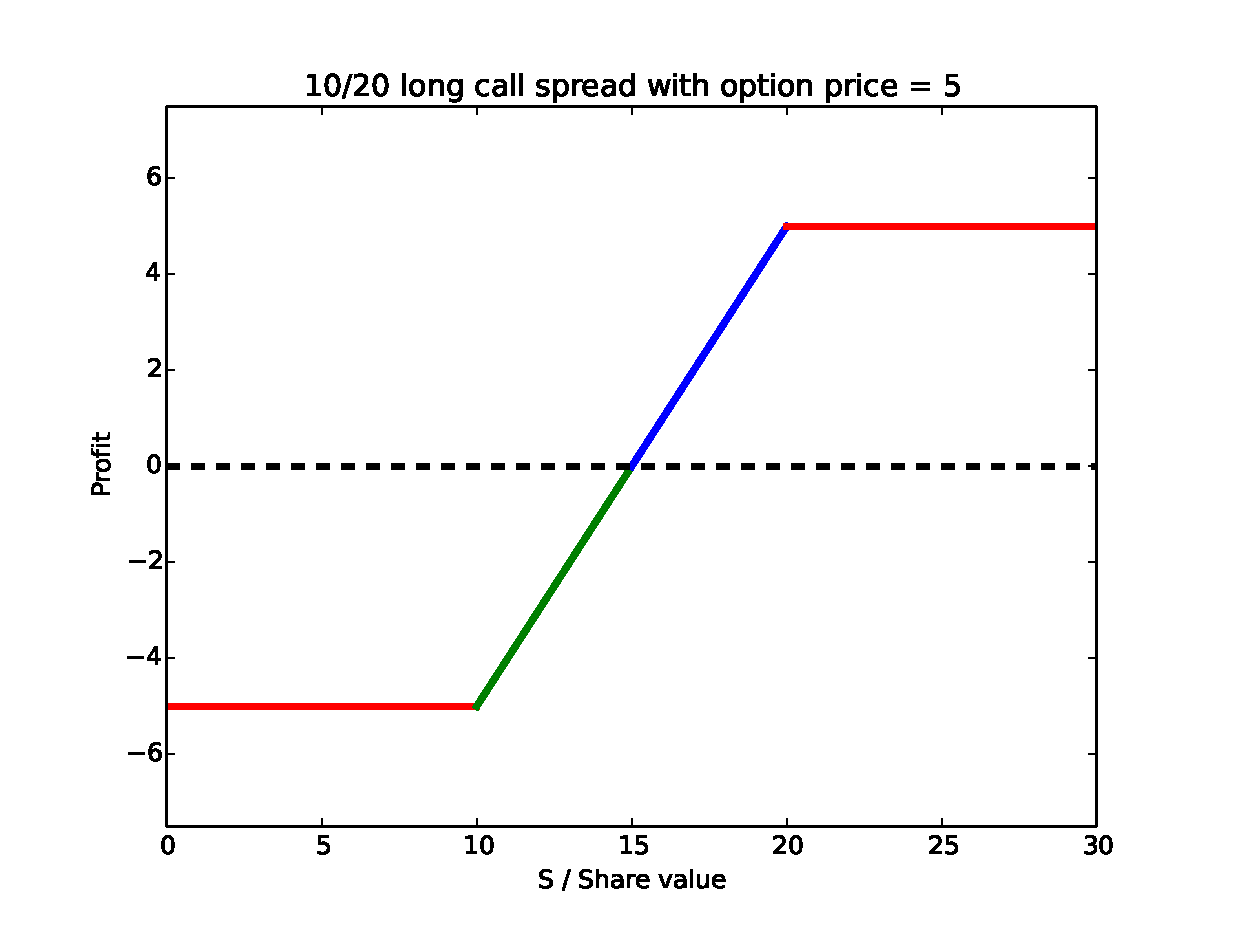
\includegraphics[width=0.8\textwidth]{graphs/long_call_option.eps}
    \captionof{figure}{Diagram of the payoff for the strategy \emph{long call option}. In this case $A=10$ and $B=20$.}
    \label{fig:long_call_option}
  \end{center}
\end{Figure}

In Figure \ref{fig:long_call_option} the pay off diagram of the long call spread is shown. There are three possible scenarios. If the stock price drops below $A$ you make a loss equal to the net amount of cash you paid for both the options. If the stock price is between $A$ and $B$ your profit is the difference between the stock price and $A$ minus the net amount paid for the options, this might still be negative. If the stock price is bigger than $B$ both options will be used. So your profit is the difference between $A$ and $B$ minus the net amount paid for the options. This is your maximum potential profit.

In the case of the 10/20 long call spread and the start stock price of 15 it would be preferable for the stock price to go up. The closer to $B$ the higher your profit will be. However, the stock price shouldn't become much higher than $B$, as profits won't increase further. But this would mean you made a bad move by putting a ceiling to your profit in exchange for a smaller loss.

\section{Put-call parity}

In a put-call parity you buy a put option, $P$, and you write a call option, $C$, with the same exercise price $E$, you also have an actual asset of the stock. So your package is: $S + P - C$. In this case you keep the options until the expiring date. At the expiring date there are two options. The stock price is smaller than the exercise price. In this case the call option will not be used, but the put option will. This makes the profit of the package $S + (E-S) - 0 = E$ minus the price of the package off course. When the stock price is bigger than the exercise price the call option will be used and the put option will not be used. Your profit is then $S + 0 -(S-E) = E$.

\begin{Figure}
  \begin{center}
    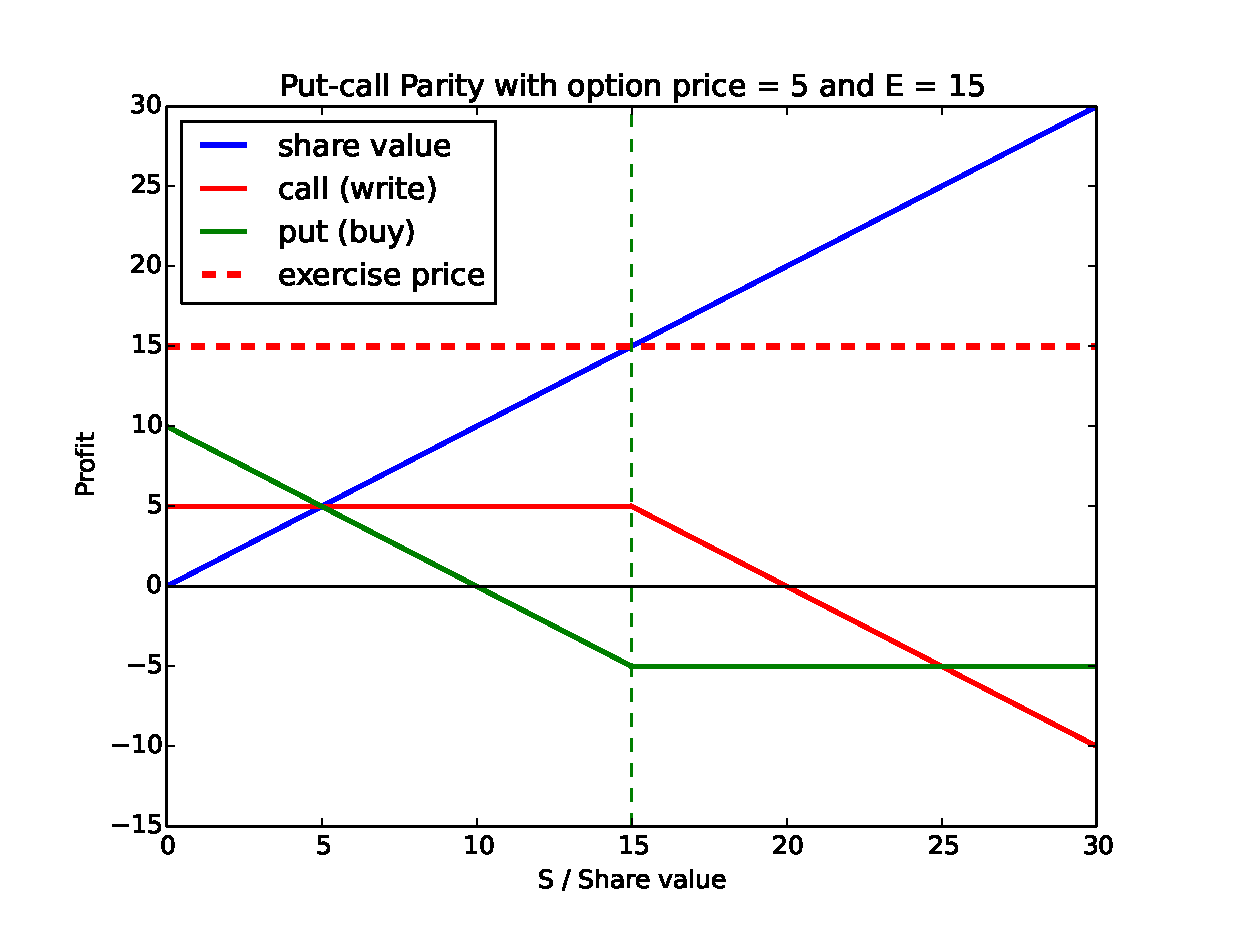
\includegraphics[width=0.8\textwidth]{graphs/put_call_parity.eps}
    \captionof{figure}{Diagram of the payoff showing the \emph{put-call parity}.}
    \label{fig:put_call_parity}
  \end{center}
\end{Figure}

In Figure \ref{fig:put_call_parity} we see that the dashed line is the profit for every value of the stock price, minus the net costs of the package, but we set that to 0 in this example. Figure \ref{fig:put_call_parity} shows that when you can acquire such a package for a price smaller than $E$ you will always make a profit.

The put-call parity formula is then

\begin{equation*}
    S + P - C = Ee^{-r(T-t)} ~~,
\end{equation*}

where $r$ represents the interest rate. This is based on the principle that having money now has more worth than having the same amount of money in the future. It is the same as discounting $S + P - C$.

\begin{thebibliography}{28}
\raggedright
\addcontentsline{toc}{section}{Bibliography}

\bibitem{Wilmott} P. Wilmott et al, \emph{The Mathematics of Financial Derivatives}, 1995.

\end{thebibliography}

\end{multicols*}

\end{document}
